\documentclass[onecolumn, draftclsnofoot,10pt, compsoc]{IEEEtran}
\usepackage{graphicx}
\graphicspath{ {images/} }
\usepackage{url}
\usepackage{setspace}
\usepackage{float}
\usepackage{caption}
\usepackage{geometry}
\geometry{textheight=9.5in, textwidth=7in}
\usepackage{listings}

\usepackage{geometry}
\geometry{textheight=9.5in, textwidth=7in}

% Taken from http://timmurphy.org/2014/01/27/displaying-code-in-latex-documents/ with some modifications
\lstset{
    frame=none,
    tabsize=4, % tab space width
    showstringspaces=false, % don't mark spaces in strings
    numbers=none, 
    commentstyle=\color{green}, % comment color
    keywordstyle=\color{blue}, % keyword color
    stringstyle=\color{red}, % string color
    basicstyle={\small\ttfamily}, % font style
    belowcaptionskip=1\baselineskip
}

% 1. Fill in these details
\def \CapstoneTeamName{		Skill Capped IRL}
\def \CapstoneTeamNumber{		17}
\def \GroupMemberOne{			Katherine Bajno}
\def \GroupMemberTwo{			Meagan Olsen}
\def \GroupMemberThree{			William Sims}
\def \GroupMemberFour{			Kiarash Teymoury}
\def \CapstoneProjectName{		eBay iOS eSports Application}
\def \CapstoneSponsorCompany{	eBay}
\def \CapstoneSponsorPerson{		Luther Boorn}

% 2. Uncomment the appropriate line below so that the document type works
\def \DocType{		%Problem Statement
				%Requirements Document
				%Technology Review
				%Design Document
				Progress Report
				}
			
\newcommand{\NameSigPair}[1]{\par
\makebox[2.75in][r]{#1} \hfil 	\makebox[3.25in]{\makebox[2.25in]{\hrulefill} \hfill		\makebox[.75in]{\hrulefill}}
\par\vspace{-12pt} \textit{\tiny\noindent
\makebox[2.75in]{} \hfil		\makebox[3.25in]{\makebox[2.25in][r]{Signature} \hfill	\makebox[.75in][r]{Date}}}}
% 3. If the document is not to be signed, uncomment the RENEWcommand below
%\renewcommand{\NameSigPair}[1]{#1}

%%%%%%%%%%%%%%%%%%%%%%%%%%%%%%%%%%%%%%%
\begin{document}
\begin{titlepage}
    \pagenumbering{gobble}
    \begin{singlespace}
    	% Need to uncomment this line below to include the COE photo
    	%\includegraphics[height=4cm]{coe_v_spot1}
        \hfill 
        % 4. If you have a logo, use this includegraphics command to put it on the coversheet.
        %\includegraphics[height=4cm]{CompanyLogo}   
        \par\vspace{.2in}
        \centering
        \scshape{
            \huge CS Capstone \DocType \par
            {\large\today}\par   
            \vspace{.5in}
            \textbf{\Huge\CapstoneProjectName}\par
            {\large CS462 Senior Software Engineering Project II}\par
            {\large Winter 2018}\par
            \vfill
            {\large Prepared for}\par
            \Huge \CapstoneSponsorCompany\par
            \vspace{5pt}
            {\Large\NameSigPair{\CapstoneSponsorPerson}\par}
            {\large Prepared by }\par
            Group\CapstoneTeamNumber\par
            % 5. comment out the line below this one if you do not wish to name your team
            \CapstoneTeamName\par 
            \vspace{5pt}
            {\Large
                \NameSigPair{\GroupMemberOne}\par
                \NameSigPair{\GroupMemberTwo}\par
                \NameSigPair{\GroupMemberThree}\par
                 \NameSigPair{\GroupMemberFour}\par
            }
            \vspace{20pt}
        }
        \begin{abstract}
        % 6. Fill in your abstract
        This document outlines the midterm progress made on the eBay iOS eSports application during winter term. Included is a discussion of the projects purpose and goals, and the progress made, remaining work, problems encountered, and interesting code of the group members based on the last six weeks.
            
        	%This document is written using one sentence per line.
        	%This allows you to have sensible diffs when you use \LaTeX with version control, as well as giving a quick visual test to see if sentences are too short/long.
        	%If you have questions, ``The Not So Short Guide to LaTeX'' is a great resource (\url{https://tobi.oetiker.ch/lshort/lshort.pdf})
        \end{abstract}     
    \end{singlespace}
\end{titlepage}
\newpage
\pagenumbering{arabic}
\tableofcontents
% 7. uncomment this (if applicable). Consider adding a page break.
%\listoffigures
%\listoftables
\clearpage

% 8. now you write!
\section{Purpose and Goals}

\subsection{Purpose}
eBay would like to make use of recently released public APIs in order to explore the eSports market and target new customers. 
Currently, there aren’t any known products that make it easy for eSports fans to find merchandise and receive updates about their favorite games. 
The purpose of our application is to showcase the new eBay APIs and attract millennial gamers. 

\subsection{Goals}
We have a few goals for our project. The first is to create an application that helps eBay learn more about the eSports market and about new shopping opportunities. The second is that our application should allow users to find and purchase eSports merchandise that is being sold on eBay. The third and final goal is to create an environment for millennial gamers to learn more about upcoming eSports events.

\section{Will}
\subsection{Progress Made}
We delegated work over break and tried to make sure that we had an equal workload among teammates. Before we started getting deep into development, I made significant UI design changes to the our application. Using Sketch, I changed the color scheme from yellow to blue and created a logo for the app. We felt the blue color scheme was more visually appealing than the yellow and it was easier to read blue text on a white background. The logo I created is a blue rupee which is used as currency in the Legend of Zelda video game series and relevant since video games are the main theme of our app. I also made significant design changes to the home screen, browse by game, sign in, register, and filter screens. This made the design more consistent throughout the entire application and assured that everyone on the team had a high fidelity design spec to follow as they implemented their screens.

I have been assigned the swiping navigation bar, Twitter functionality, and featured events. During winter break, Kia and I worked together to implement the swiping navigation bar with a UIViewController that uses UICollectionViewControllers as pages. Once Kia and I finished the navigation bar, I added the required UICollectionView cells that would be displayed on the homescreen. The Featured\_Events cell is what will eventually contain the title, date, and location of chosen featured event. Currently, I have added the carousel that Katherine made which will eventually display items being sold on eBay associated with the featured event. I have also added the button which is labeled “See more” that will eventually allow users to navigate to the associated browse screen for the event so that they can purchase related merchandise being sold on eBay.

I have also successfully implemented the Twitter\_Cell and it currently displays a tweet from Overwatch League. Below the tweet, I added a “See more tweets” button which navigates the user the twitter timeline for the same account as the single tweet. The timeline was implemented using a TWTRTimelineViewController and a delegate so that the view controller can be pushed when selecting a button in the twitter cell. This functionality was implemented using guest authentication and the official Twitter API and iOS Kit. The Header\_Cells were added to separate the “Featured Events” and “Favorites” areas. I added a blank UICollectionViewCell for the favorites which will be finished by Katherine in the future. 

\subsection{Remaining Work}
I have made a lot of progress on the pieces of the app that I have been assigned, but there is still work that needs to be completed before expo. The Twitter functionality is almost entirely complete, I just need to implement a way to grab the most recent tweet of a targeted account when the app is launched. Currently, the Tweet displayed is static, but I should be able to retrieve the most recent Tweet ID from an account using a GET statuses/user\_timeline request with the API. The last thing I will need to implement for Twitter is a way to dynamically size the Twitter\_Cell depending on the tweet retrieved. I have played around with the sizeThatFits() function and I will use it to retrieve the correct height the tweet view so that it is correctly displayed in the app.

In order to finish the featured events cell, I will need to the title, date, and location of the featured event to be displayed. I have chosen to use E3 as our featured event for expo so I will just need to implement the necessary subviews to be displayed in the Featured\_Events\_Cell. I have downloaded a high fidelity graphic for the E3 banner which will be added to the cell as well. I will also need to work with Kia to populate the carousel with items being sold on eBay that are related to the E3 expo. We will want to display merchandise related to E3 and the video games that will be displayed there. The icons I created for the date, time, and see more buttons will need to be imported into the project and added to the home screen as well. I also plan to make some small improvements to the logo being displayed above the navigation bar because it is currently larger than what I had created in my design.

Lastly, I will need to spend some time refactoring my code so that it is easier to read and effectively follows the MVC design pattern. Overall, I am confident that I can finish the work assigned to me before the deadline for our project.

\subsection{Problems Encountered}
Since this is my first time building an iOS app and developing in Swift, I’ve run into a few problems as I’ve learned the platform. I had difficulties choosing what type of view controller and views to use for the home screen, but eventually decided on collection views since they have many properties that can be changed in order to make them function exactly how you want. I’ve been using the YouTube channel “Lets Build That App” as a resource for learning Swift and so far it has been going well.

I had some issues getting twitter to authenticate properly, but it turns out that I had accidentally left a comment in the Info.plist file which was causing the error. Another small inconvenience that I’ve encountered is that when running our application, I get the warning that Twitter Kit for iOS has duplicate installations. I’ve researched the warning and according to the Twitter developer forums is in an issue caused by a recent update for CocoaPods. The warnings don’t stop the app from running properly, but hopefully there will be an update soon that will resolve the issue.

Another problem that I’ve encountered is getting the dimensions of the tweet view cell before displaying the cell in my view controller. With the way I currently display Tweets, it is all done in the collection view and therefore I set the height of the cell before I know the size of my tweet. In order to solve this issue, I plan to implement a Twitter model class where the height of the cell is determined and passed to the view controller prior to displaying the tweet. This will allow me to dynamically size the cells for when I implement most recent tweets instead of static tweets. 
\subsection{Interesting Pieces of Code}
\noindent\textbf{Loading a single tweet to be displayed.}
\begin{lstlisting}
// Create Twitter client and load the tweet with a specific ID
let client = TWTRAPIClient()
client.loadTweet(withID: "959124212198686720") { (tweet, error) in
  if let t = tweet {
    self.tweetView.configure(with: t)
    self.setTweetSize(t:self.tweetView)
  } else {
    print("Failed to load Tweet: \(error?.localizedDescription)")
  }
}
\end{lstlisting}
\noindent\textbf{Twitter Timeline View Controller}
\begin{lstlisting}
class Twitter_Timeline: TWTRTimelineViewController {
    override func viewDidLoad() {
        super.viewDidLoad()
        title = "Overwatch League"
        self.dataSource = TWTRUserTimelineDataSource(screenName: 
"overwatchleague", apiClient: TWTRAPIClient())
    }
}
\end{lstlisting}

\subsection{User Interface Designs}
\begin{figure}[H]
\centering
\captionsetup{justification=centering}
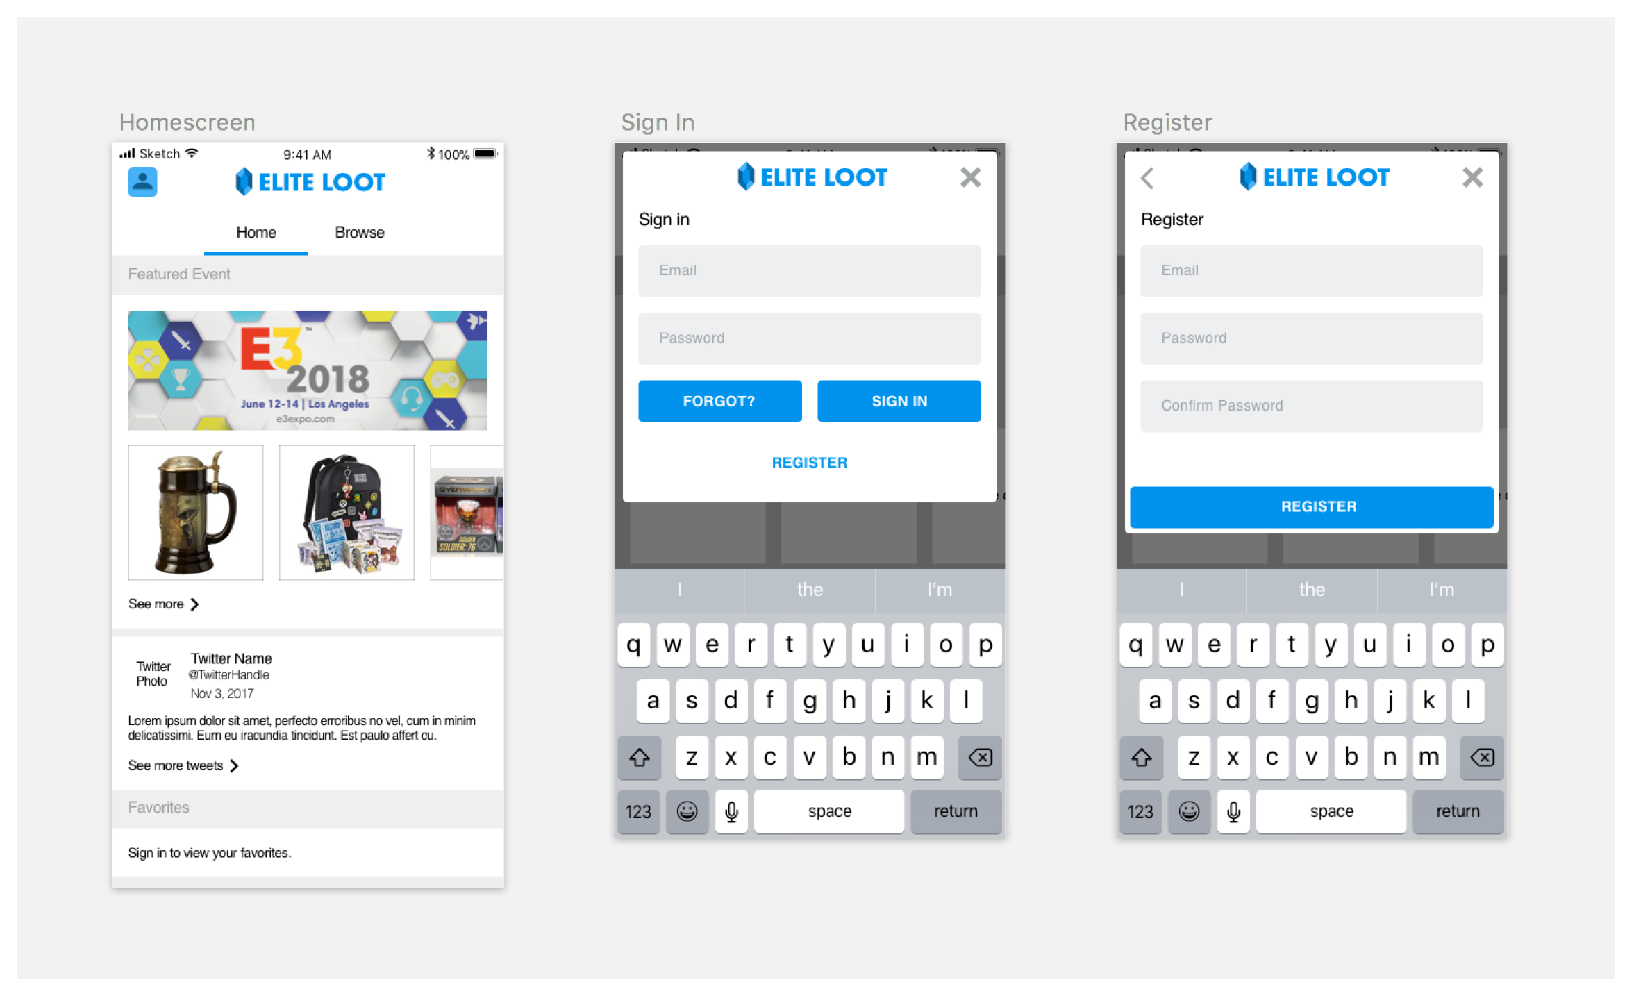
\includegraphics[scale=.50]{homescreen}
\caption{Updated designs for home screen, sign in, and register.}
\end{figure}

\begin{figure}[H]
\centering
\captionsetup{justification=centering}
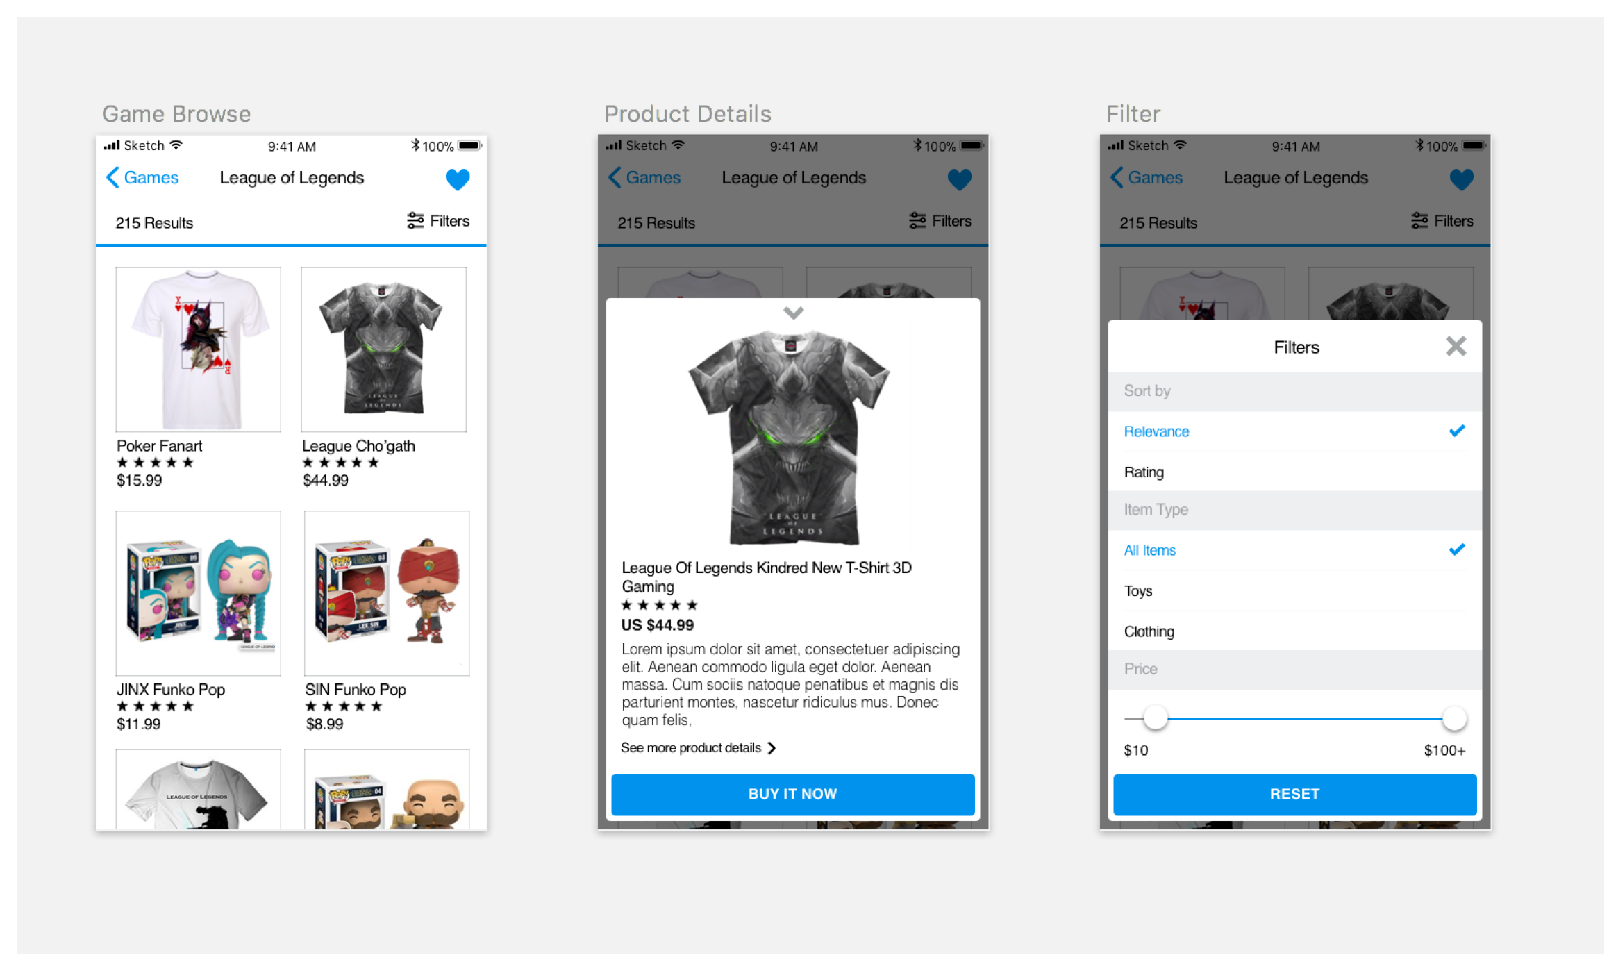
\includegraphics[scale=.50]{browse_game}
\caption{Updated designs for browse game, product details, and filter.}
\end{figure}

\section{Kia}
\subsection{Progress Made}
\par After we successfully got through the first term, we were able to divide up the work equally among everyone on the team to avoid any extensive workload for any team members. Prior to the winter term, Will and I met few times to talk about our design concepts and things we could further accomplish with the app. We also talked about the way we could implement the navigation bar on the main page. We ended up working on it over the break to get it fully working the way we wanted. Eventually going into the winter term, for the first couple of weeks, I tried to mostly focus on the shell of the pages I was assigned. Since a lot of the screens assigned to me are mostly reusable, I tried to come up with ways to implement something that could be re-used throughout all the pages of the application. I first looked into how I could create a grid of items to display the retrieved merchandise and using UICollectionViews seemed to be the best approach for this. I used a UIImageView along with a UITextView to display the details for each merchandise image along with their given summaries. 
\par To make sure I had everything set up correctly, I then created some dummy data to test this page. My second step was to create the buy item page along with filtering and sorting that open modally from the bottom. Since both of these pages had the same animation, I had to make sure I create a model to use for both. The solution I came up with eventually was to create a parent page as the base view and use an initializer to populate the page the user is requesting. In addition, I also had to create two different UIView classes, one being a TableView and another just being a normal UIView to display the attributes for each page. I didn't want to create another ImageView and UITextView for the item details screen. Therefore, I inherited from the cell class and used encapsulation to override the layout methods. This way I had control over how and where I wanted everything placed. Finally, I created a model object for each section of filter-sorting using enums which made it easy «to display each section with the number of rows and have that page be presented the way I want. 
\par The very last thing I’ve been working with after finishing most of the layout is implementing the eBay Browse API. Since our main objective for this application was to test this beta API, I had to make sure the way I implement this is fully efficient and every request needed is fully handled. It took me one whole day just to understand how the API works and how it needs to be implemented. After some more research, I was successfully able to request data by querying the item names and use the JSON decoding protocol provided by Apple to get a model object and update the main UI. I Also sent another HTTP request to download the images for each item that has an image URL associated with it.
\subsection{Remaining Work}
\par Over the past 6 weeks, I have finished more than 75 percent of the assigned work. With eBay API fully implemented and shell ready to use, my next plan is to finish the remaining of the filter page where users could sort and query the data based on their preference. There is also some stuff with calling the API that I like to do to improve the performance and efficiency of the request. Once everything is done regarding the eBay request Im also planning on going back and look at things that could further be refactored and reused.  There is some cell sizing that I need to implement based on the items names and details. This way I could make sure that there is no text overlapping and every device size is fully supported. Finally, once I have everything working with the eBay API, I will try to create a handshaking framework to check the status of the token before retrieving data since the token expires every couple of hours. 

\subsection{Problems Encountered}
\par One of the problems I encountered at the beginning of development was definitely when creating the navigation between each page. Will and I thought using a PageViewController would be the best choice. However, after working with it and trying to create the transition for the slider between each page, we figured that we had an issue and we couldn’t get it to work. We ended up fully changing the implementation and coming up with a better solution to create this transition between each page using UIScrollView. 

\par One problem that I am still having is refreshing my token before the request. Currently, the token has to be refreshed every few hours to retrieve data. I still yet have to figure out how I could get a hold of the token with HTTP requests without having to update it myself. eBay expires the token every few hours for the privacy of its users which could create some conflicts. The last thing I struggled with a bit was to find out how I could get a category ID associated with each merchandise. I had to look for specific items to find the pattern between each Id to come up with my solution. I later found out that there is another request that could be made to get each category that Item has along with all of their unique ids. 

\subsection{Interesting Pieces of Code}
\noindent\textbf{Browse API URL Endpoint.}
\begin{lstlisting}
private var endPoint: URL? {
    let baseUrl = "https://api.ebay.com/buy/browse/v1/item_summary/search?",
        query = "q=\(keyWord ?? "")&",
        groupBy = "category_ids=\(groupingBy?.rawValue ?? "")&",
        limit = "limit=30&",
        buyOption = "buyingOptions%3A%7BFIXED_PRICE%7D",
        condition = "conditions%3A%7BNEW%7D&",
        filter = "filter=\(buyOption),\(condition)",
        sort = sortBy?.rawValue ?? ""
    return URL(string: baseUrl + query + groupBy + limit + filter + sort)
}
\end{lstlisting}
\noindent\textbf{Browse HTTP request}
\begin{lstlisting}
func requestData(forUrl url: URL, completion: @escaping (RequestRespnse, Model?) -> ()) {
    let authString = "Bearer \(token)"
    let config = URLSessionConfiguration.default
        config.httpAdditionalHeaders = ["Authorization" : authString]
    let session = URLSession(configuration: config)

    let task = session.dataTask(with: url) {
        (dataObj, respnse, error) in
        guard       error == nil,
                let data = dataObj else { return completion(.error(error?.localizedDescription ?? ""), nil)  }

        completion(.success("Successfully Requested Data"), self.decode(data: data))
    }
    task.resume()
}
\end{lstlisting}   

\section{Meagan}
\subsection{Progress Made}
\par By the end of fall term, we had divided up the responsibilities between the four members of our team. Since most of the team shared a common interest in front end development, we thought it would be most fair to divide up the project in such a way that each person would contribute to both the front end and back end of our application. After fall term, my responsibilities included the log in/log out screen, register screen, implementing the actual authentication using Firebase Auth, and displaying the details for a specific item on our browse specific item screen. With the responsibilities divided up, we had a shared consensus among the team to at least get started on the build of our project over winter term. 
\par For me personally, knowing my responsibilities, I decided to start with the Firebase authentication since that was the task that I was most excited about. Since I didn’t know anything about Google’s Firebase, I decided to go into the Portland eBay office to kind of a proof of concept glimpse as to how Firebase actually worked within the context of an application. At the beginning of the project, our team was assigned four mentors as a resource to kind of help us out with the different technical aspects of the project. Each of the mentors had a different skill set, so I had to find the one with knowledge of the authentication. When I went into the office, he was able to direct me to the resources needed to setup the project with Firebase as a first step. This included creating a new project in Firebase, allowing for authentication, and configuring Firebase with our project by setting up the Firebase SDK and installing the necessary pods. During this time, I also created my own separate project to walk though a tutorial to which I was redirected to by one of the eBay mentors. This tutorial was incredibly useful, because it also demonstrated how to use Firebase to store other types of data although the data for our project hadn’t specifically been defined at this point. I was able to finish most of the tutorial on a separate project of my own before I ran into a stopping point. I didn’t get as far as I would have liked to on the actual implementation over break, but I did take advantage of my convenient access to the eBay mentors while I was back in Portland and was able to acquire some great resources as well as see a proof of concept of the authentication part of the application in action.
\par At the beginning of winter term, I was very ambitious to get started because I knew that I would have an incredibly busy term later in the term. So, within the first few weeks, I dedicated my weekends and evenings to the project, reading documentation and trying to determine how I was going to implement my assigned pages. By the third week, I had read all of the Swift documentation on the Apple website and had implemented a sign in and registration page relying on Firebase to handle the entire back end including storing and managing users with separate hashes. However, since our group had still not finalized our designs, I found that my approach to implementation was wrong, and so I had to re implement the views that I had already created differently.  I am currently nearly finished with the sign in page and still needing to implement the registration page. I also met with my teammates, and we explicitly mapped out the data model. This is the current state of where I am now. 

\subsection{Remaining Work}
\par In order to stay on track with the recommended schedule of the project as described in class, I need to have my UI components finished by the end of this week(week 6). This should be doable as the registration page should be trivial once the sign in page is complete. I also still have to finish up the last small piece of the sign in page, but after that it should be trivial as there is only one last piece that needs to be changed, and I now know what needs to be done to fix it. 
\par The next week (week 7), my plan is to start implementing the database storage in Firebase for the favorites since that is an immediate need of my teammate Katherine to move forward with implementing her part. Since I do have a feel for how this should be done from the tutorial that I worked on over winter break, I already have a starting ground for this. However, to be extra cautious, I plan to start on this as early as possible to make sure to give myself plenty of time for any problems that might arise. 
\par The last part of my portion that needs to be done is implementing the methods to manually handle the authentication using Firebase. Thankfully, I have already walked through these methods in the tutorial on my other project, so I also have a starting ground for this. As far as displaying a specific item goes, that is already up and running as my teammate Kia actually took on that task while he was implementing the eBay browse API.  
\par Finally, any additional time that I have left will be used for extensive testing and fixing little things with the UI views. My plan is to also work on this project over Spring break too in order to give me extra time to clean it up better. 

\subsection{Problems Encountered}
\par Perhaps the largest problem that I encountered was the incorrect implementation of the original sign in and registration pages. This was partially my fault as I wasn’t as assertive in communicating with the team throughout the development of this part of the project.  My team has one teammate who has done iOS development before, but the rest of us are completely new to it. Not having this experience made it difficult for me to understand when my teammate was trying to explain the way that we had chosen to do it.
\par Another problem that I faced early on is when I first tried to pull down the code and compile it. I faced many linker errors. This was fixed from simply re cloning the project. Another issue that I ran into during development was a merge conflict the first time I tried to push my code for the user interfaces for the sign in and registration page. This was easily fixed by pulling down the code and comparing the version from my branch with master. I realized that it was a silly error and that I had forgotten to fetch before I tried to merge my code. 
\par The last issue that I faced was when I went back and reimplemented the sign in page. The first input box was getting partially cut off for some reason, and I couldn’t figure out why. This was easily solved in the next meeting I had with my team in which we figured out that it was actually the logo at the top of the sign in page that was causing this problem. My team helped me out my removing the border from the logo so that it hopefully has a smaller surface area and doesn’t cut off that top input box.

\subsection{Interesting Pieces of Code}
\begin{lstlisting}
let emailContainerView : UIView = {
    let emailContainerView = UIView()
    emailContainerView.backgroundColor = UIColor(r:220,g:220,b:220)
    emailContainerView.translatesAutoresizingMaskIntoConstraints=false
    emailContainerView.layer.cornerRadius = 4
    emailContainerView.layer.masksToBounds = true
    return emailContainerView
    }()
\end{lstlisting}
\par This piece of code essentially sets up a container for the email input box on the sign in page. 
\begin{lstlisting}
view.addSubview(emailContainerView)
\end{lstlisting}
\par This code then adds the view itself to the new blank page.
\begin{lstlisting}
 func setupEmailViewContainer(){
 //setup constraints
emailContainerView.topAnchor.constraint(equalTo: signInTextField.bottomAnchor, constant: 15).isActive = true
emailContainerView.leftAnchor.constraint(equalTo: view.leftAnchor, constant: 23).isActive = true
emailContainerView.widthAnchor.constraint(equalTo: view.widthAnchor,constant: -30).isActive = true
emailContainerView.heightAnchor.constraint(equalToConstant: 50).isActive = true
\end{lstlisting}
\par This code then positions the container where we want it on the page. These pieces of code are particularly interesting because this is a repeated pattern for how all of the UI elements are dimensioned on the page, and it is in contrast to the way other platforms such as Android do it with a separate XML file and such.

\section{Katherine}
\subsection{Progress Made}
In these last six weeks, I have been working on getting the user interface of the browse screen set up. It has proved to be more challenging than I originally thought it would be. During weeks one and two, I spent most of my time researching and gathering resources for the development of my browse screen. My research was mainly focused on my options for getting the merchandise carousel implemented, as the code for it will not only be used for my browse screen, but for other team members portions as well. I watched YouTube tutorials and read documentation to determine what would be the best view to use. Through my research and discussion with my team members, I determined that a UICollectionView is what I wanted to use. Another thing I accomplished during these weeks was finalizing the design for the browse screen in Sketch.

\par After the research was done, my remaining weeks were spent learning how to program a user interface using Swift and getting the shell for the browse screen completed. Through much trial and error, I was able to successfully implement the shell. To accomplish this task, I ended up using three nested UICollectionViews. The main UICollectionView has two cells. This cell contains a subview for the image on top, and another UICollectionView for the bottom half for the carousel. The second UICollectionView contains just one cell. It stores another UICollectionView, which is the carousel. It contains as many cells as there are items to display, in this case five for browse events and seven for browse games.

\subsection{Remaining Work}
I still need to finish implementing the browse screen and the favorite game feature. My next step is to gather up the images that will be used for the browse events and browse games headers, and get them stored into the Firebase. After gathering the images necessary, I will speak with Meagan about getting them stored in the Firebase as that is her responsibility. I will be able to populate these images that are contained in separate UICollectionViews from the Firebase to be displayed on the view for the user.

\par After I am able to get these images displayed, the next thing I will work on is the favorite game feature of our application. This feature allows the user to favorite and unfavorite a game on the browse screen. Each of the 10 games in the browse games UICollectionView carousel will contain a blue heart on it. I need to figure out how I will get this blue heart to display and be touchable. If the heart is filled in, it means a user has favorited that game. If the heart is empty, the game is not in the user’s favorites. In-order to determine this, I will need to check the user’s favorites based on their unique ID in Firebase when they are signed in. A modal will be displayed when the user favorites and unfavorites a game to alert the user of the action they completed. I also need to implement error-handling for this feature. To favorite an item, a user needs to be signed in. If they are not, a modal will prompt them to sign in to check their favorites and to add more favorites. 

\par After implementing the modal, I need to display the user’s favorite games on the home screen. First, I must check if a user is signed in or not. If they are not signed in, a message will be displayed under favorites letting the user know to sign in so they can customize this area of the screen. If a user is signed in but contains no favorites, a message informing them that they are able to favorite items by tapping on the blue heart on the browse screen will be in place of the favorites. If a user is signed in and also has favorited games, then the favorites section will be populated with the games and relevant merchandise using their unique user ID stored in the Firebase to access their data. There will be as many cells as the user has favorite games. Each cell will contain a thumbnail image and title of the game, and a carousel of merchandise they can purchase relevant to the game.

\par Another task that I need to complete is linking the events and games displayed by the carousel’s in the browse screen to the correct screens. When a user selects an event or game, they should be taken to another screen where they can browse merchandise relevant to the event or game selected. From there, they can filter merchandise by clothes or toys and also make purchases. The merchandise screen will be done by Kia. I need to make sure that when the user makes a selection, the next screen contains the correct event or game.

\subsection{Problems Encountered}
The initial problem I encountered was my lack of iOS knowledge. After first downloading the repository from GitHub onto my computer, I struggled to get the project up and running. To fix this issue, I spoke with my team and they led me in the right direction. The issue was solved by updating my CocoaPods file in my project folder on my computer. After getting the project up and running, I had a problem figuring out where to start. Since Will and Kia had begun the initial interface, I had something to work with. Will pointed me to a YouTube channel titled "Let's Build That App" where there are great resources for building iOS applications. So to solve my problem, I followed along with a YouTube clone tutorial on the channel. This taught me how the various screens were set up on an iOS application.

\par When implementing the UICollectionViews on the browse screen, I ran into an issue of how to split up the initial cells. I knew I needed an image as a header, and multiple cells for the carousel. I first explored subviews. I had a subview for the image on top, and a subview for the bottom items. I then attempted to just place the second UICollectionView directly into the first UICollectionView. While this worked, the second UICollectionView was centered vertically in the first one. I spent two hours trying to get the second one to anchor to the bottom and failed. The issue was that since the first UICollectionView took up the entire cell, the second UICollectionView would position itself based on the first view and not the subviews within the view.

\par Upon discovering this, I decided to try nesting three UICollectionViews instead of two. The second one would be anchored to the bottom with the correct size below the image header, and the third UICollectionView would be contained within the second one. This worked great as soon as I tried it. It was no longer a challenge to center the carousel of items. Since the correct sizing was done in Sketch beforehand, I did not have to play with the sizing of the cells. It was an easy fix once I had located my issue.

\subsection{Interesting Pieces of Code}
\noindent\textbf{Creating a UICollectionView for item carousel.}
\begin{lstlisting}
 let itemsCollectionView: UICollectionView = {
        let layout = UICollectionViewFlowLayout()
        layout.scrollDirection = .horizontal
        let collectionView = UICollectionView(frame: .zero, collectionViewLayout: layout)
        
        collectionView.backgroundColor = .clear
        collectionView.translatesAutoresizingMaskIntoConstraints = false
        collectionView.showsHorizontalScrollIndicator = false
        
        return collectionView
    }()
\end{lstlisting}

\noindent\textbf{Inserting a UICollectionView as a subview.}
\begin{lstlisting}
 addSubview(itemsCollectionView)
        
        //to generate multiple cells in nested collection view
        itemsCollectionView.dataSource = self
        itemsCollectionView.delegate = self
        
        //register item cell to the collection view
        itemsCollectionView.register(ItemCell.self, forCellWithReuseIdentifier: cellId)
        
        //expand from left to right edge
        addConstraints(NSLayoutConstraint.constraints(withVisualFormat: "H:|-15-[v0]|", options: NSLayoutFormatOptions(), metrics: nil, views: ["v0": itemsCollectionView]))
        
        //expand from top to bottom
        addConstraints(NSLayoutConstraint.constraints(withVisualFormat: "V:|[v0]|", options: NSLayoutFormatOptions(), metrics: nil, views: ["v0": itemsCollectionView]))
\end{lstlisting}


\subsection{User Interface Designs}
\begin{figure}[H]
\centering
\captionsetup{justification=centering}
\includegraphics[scale=.50]{browsescreen}
\caption{Updated design for the main browse screen.}
\end{figure}

\section{Conclusion}
Overall, we have made significant progress on our application and we are confident that we can meet all of our requirements prior to the code freeze. As a group, we need to figure out how we will organize our Firebase data tables since it will be used by multiple teammates. The eBay browse API and Twitter API implementation is nearly complete. Only small features are left such as dynamic tweets and filtering. The main tasks that remain on our project involve implementing the user interface to match the designs and utilizing Firebase data storage to retrieve content.  

\end{document}

